\FloatBarrier
\begin{figure}[!h]
\centering
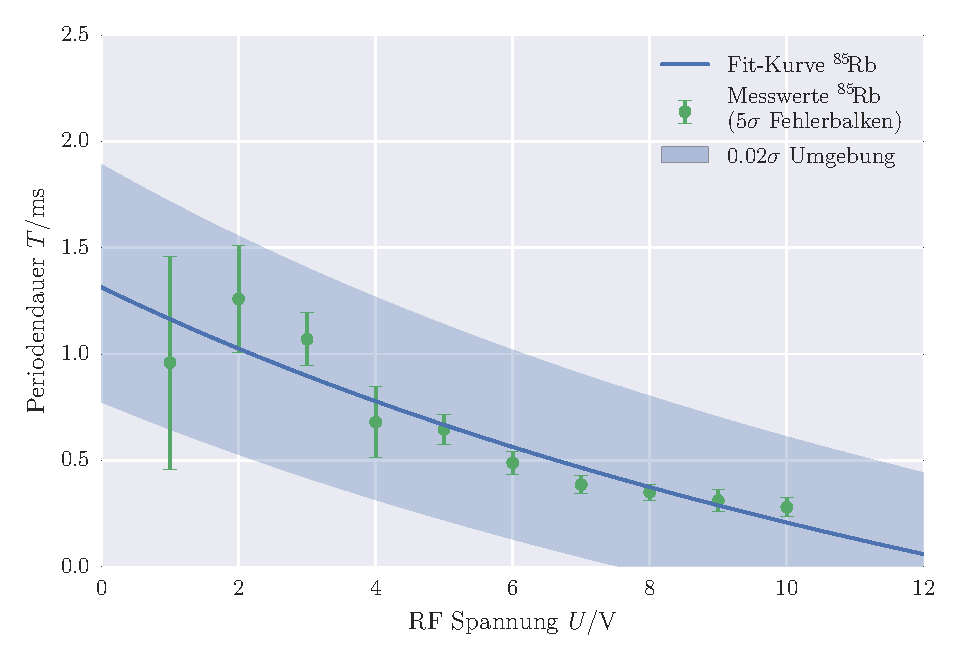
\includegraphics[scale=.8]{../Grafiken/Transienteneffekt_Rubidium_85.pdf}
\caption{In Abhängigkeit der RF-Spannung dargestellte Periodendauern der Relaxation
	für das Isotop ${}^{85}\!$Rb. Die Fehlerbalken der Messwerte wurden verfünffacht, 
	um sichtbar zu sein. Zusätzlich ist die hyperbolische Ausgleichskurve für die Messwerte
	dargestellt. Bei dem abgebildeten Fehlerbereich der Ausgleichskurve handelt es sich nur 
	um einen Bereich mit $\sfrac{1}{50}$ der eigentlichen Größe. Dieser große Fehler ist durch 
	den ersten Messwert bedingt. \label{fig:transienteneffekt_rubidium_85}}
\end{figure}
\FloatBarrier